\chapter{Obsah paměťového média}
\dirtree{%
.1 /\DTcomment{Médium}.
.2 aux/\DTcomment{Pomocné soubory}.
.3 density/\DTcomment{Odhad a generování pst. rozdělení}.
.4 in/\DTcomment{Převzaté zdrojové soubory algoritmů}.
.4 out/\DTcomment{Grafy pravděpodobnostních rozdělení}.
.4 src/\DTcomment{Skripty pro odhad a generování pst. rozdělení}.
.3 scalability/\DTcomment{Zkoumání škálovatelnosti}.
.2 models/\DTcomment{Převod modelů z Verilogu do UPPAAL}.
.3 out/\DTcomment{Výstupní XML soubory -- systémy modelů programu UPPAAL}.
.3 templates/\DTcomment{Šablony jednotlivých modelů}.
.3 verilog/\DTcomment{Vstupní soubory -- modely násobiček ve Verilogu}.
.3 parse.py\DTcomment{Skript pro překlad modelů z Verilogu do UPPAAL}.
.2 results/\DTcomment{Zpracování výsledků simulací}.
.3 out\_csv/\DTcomment{Zpracované výsledky ve formátu csv}.
.3 pickles/\DTcomment{Pandas DF uložené v souboru pkl obsahující výsledky simulací}.
.3 plots/\DTcomment{Grafy výsledků simulací}.
.3 sim\_results/\DTcomment{Výsledky simulací ve formátu csv}.
.3 plot\_results.py\DTcomment{Skript pro vytvoření grafů}.
.3 print\_results.py\DTcomment{Skript pro vytvoření výstupních csv souborů}.
.3 process\_results.py\DTcomment{Skript pro vytvoření Pandas DF z csv výsledků simulací}.
.2 thesis/\DTcomment{Zdrojové soubory textu}.
}

\chapter{Návod na zprovoznění}
V této příloze je popsáno, jak zprovoznit program UPPAAL, jak pracovat se skriptem pro překlad modelů a jak spouštět simulace v prostředí UPPAAL.

\section*{Nástroj UPPAAL}
Pro provádění simulací je zapotřebí nainstalovat simulační nástroj UPPAAL. V době vzniku této bakalářské práce byla aktuální verze 5.0.
Program lze stáhnout na adrese \url{https://uppaal.org/downloads/} v závislosti na operačním systému. Dále je nutné se zaregistrovat na adrese \url{https://uppaal.veriaal.dk/academic.html} pro obdržení licence k používání programu. Pro akademické pracovníky a studenty je zdarma.

\section*{Skript parse.py}
Pro spouštění skriptu je potřeba prostředí \texttt{python3}. Ve skriptu jsou použity pouze standardní moduly \texttt{re} a \texttt{argparse}.

Skript lze spouštět v příkazové řádce ve tvaru
\begin{equation*}
    \texttt{python3 parse.py input\_file [-d DISTRIBUTION] [----noout]}.
\end{equation*}
Argumenty skriptu mají následující význam:
\begin{itemize}
    \item \texttt{input\_file} je cesta ke vstupnímu souboru s modelem násobičky napsaným ve Verilogu,
    \item \texttt{-d DISTRIBUTION} je nepovinný argument sloužící pro specifikaci vybraného pravděpodobnostního rozdělení pro generování vstupů. \texttt{DISTRIBUTION} může být jeden z názvů rozdělení popsaných v části \ref{zvolene_aplikace},
    \item \texttt{----noout} je nepovinný přepínač sloužící k případnému zakázání vytváření výstupního XML souboru. Vhodné pouze k ladění skriptu.
\end{itemize}
Výstupní soubory se v aktuální podobě skriptu ukládají do složky \texttt{./out}, která má uvnitř téměř stejnou strukturu, jako složka \texttt{./verilog} obsahující vstupní soubory.

\section*{Simulace}
Soubor vygenerovaný skriptem \texttt{parse.py} je možné otevřít v programu UPPAAL. V části programu nazvané \texttt{Verifier} jsou připraveny simulační dotazy. Jednotlivé dotazy lze spouštět tlačítkem \texttt{Check}. Po dokončení simulace lze na dotaz kliknout pravým tlačítkem myši a poté kliknout na položku \texttt{Simulations (1)} pro otevření vizualizace výsledků dané simulace. Odtud lze exportovat data ve formátu csv. Simulace posledního dotazu může trvat až několik desítek minut či jednotek hodin v závislosti na výkonu procesoru, velikosti operační paměti a také na počtu logických hradel zkoumané násobičky.

\chapter{Pravděpodobnostní grafy při odhadu max. nebo min. hodnoty} \label{append:prob_plots}
V této příloze jsou uvedeny příklady grafů popsaných v části \ref{uppaal_smc_queries}.

\begin{figure}[H]
    \centering
    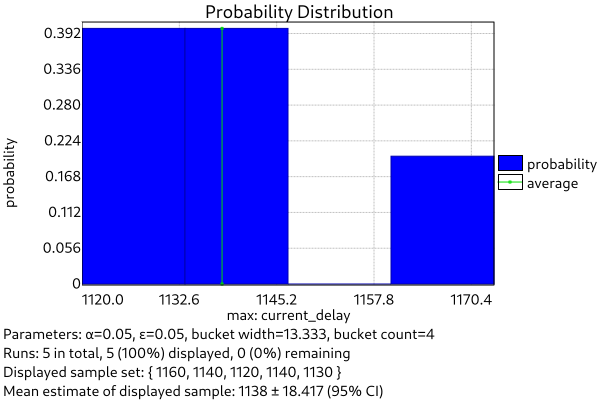
\includegraphics[width=0.75\textwidth]{obrazky-figures/plot_prob_dist.png}
    \caption{Příklad grafu rozdělení pravděpodobnosti}
    \label{fig:plot_prob_dist}
\end{figure}

\begin{figure}[H]
    \centering
    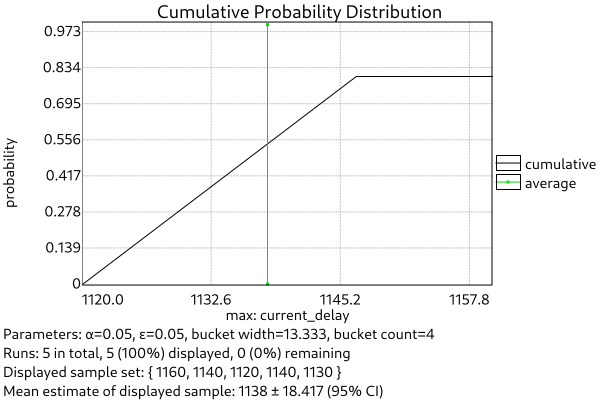
\includegraphics[width=0.75\textwidth]{obrazky-figures/plot_cum_prob_dist.png}
    \caption{Příklad grafu rozdělení distribuční pravděpodobnosti}
    \label{fig:plot_cum_prob_dist}
\end{figure}

\begin{figure}[H]
    \centering
    \includegraphics[width=0.75\textwidth]{obrazky-figures/plot_conf_ints.png}
    \caption{Příklad grafu konfidenčních intervalů distribuční funkce}
    \label{fig:plot_conf_ints}
\end{figure}

\begin{figure}[H]
    \centering
    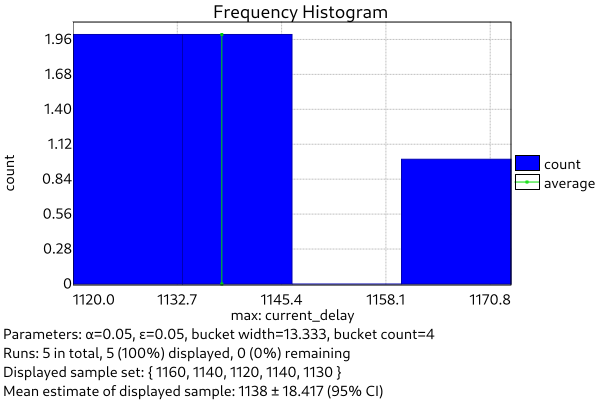
\includegraphics[width=0.8\textwidth]{obrazky-figures/plot_freq_hist.png}
    \caption{Příklad histogramu frekvencí výskytu jednotlivých hodnot při simulačních bězích}
    \label{fig:plot_freq_hist}
\end{figure}

\chapter{Pravděpodobnostní rozdělení při generování vstupů korespondující se zvolenými aplikacemi} \label{append:rozdeleni_pst}
Výchozím a referenčním rozdělením bylo zvoleno rozdělení nazvané \textbf{uni\_uni}. Oba vstupy jsou v tomto případě generovány s rovnoměrným rozdělením v intervalu 0 až 255 (minimální a maximální hodnoty, kterých může nabývat 8bitový bezznaménkový integer). Jinými slovy všechny vstupní kombinace mají stejnou pravděpodobnost výskytu.

V této sekci jsou postupně představeny jednotlivé algoritmy a získaná rozdělení. U každého algoritmu se nachází obrázek s grafy naměřených rozdělení. Struktura těchto obrázků je následující:

V grafech \textbf{(a)} a \textbf{(b)} je vidět hustota rozdělení pravděpodobnosti (zkr. PDF z angl. \textit{probability density function}) získaná z reálných naměřených dat z algoritmů. V grafu (a) je zobrazena pravděpodobnost výskytu pro oba vstupy zvlášť, v grafu (b) je to stejné v podobě teplotní mapy. V grafech \textbf{(c)} a \textbf{(d)} jsou zobrazena výsledná odhadnutá pravděpodobnostní rozdělení pro oba vstupy.

Dále je u každého algoritmu vypsán pseudokód generování čísel dle zvolených rozdělení. Součástí kódu ve výsledném souboru pro nástroj UPPAAL je mj. i ošetření překročení hranic (čísla menší než 0 se nastaví na 0, čísla větší než 255 se nastaví na 255), které v pseudokódech není zahrnuto.

\pagebreak

\subsubsection{Algoritmus Ellipse Mid-Point}
Ellipse Mid-Point je algoritmus používaný v grafice pro rasterizaci elipsy. Na obrázku \ref{fig:beta_uni} jsou znázorněna pravděpodobnostní rozdělení vstupů násobičky. Pseudokód zvolených rozdělení je následující:

\begin{lstlisting}[language={C}, label={lst:ellipse}]
input_x = int(random_beta(0.5, 5.0) * 40)

input_y = int(random_uniform(0, 266))
if input_y > 255:
    input_y = int(random_uniform(0, 15))

if input_y < 2:
    input_y += 2
\end{lstlisting}

Pro generování vstupu X bylo zvoleno rozdělení beta s parametry $\alpha = 0,5$ a $\beta = 5$ následně vynásobené hodnotou 40. Vstup Y je generován mírně deformovaným rovnoměrným rozdělením od 0 do 255. V rámci experimentů byla tato dvojice rozdělení označena jako \textbf{beta\_uni}.

\begin{figure}[H]
    \centering
    \includegraphics[width=0.85\textwidth]{obrazky-figures/beta_uni_all.png}
    \caption{(a) a (b) PDF násobených dvojic rasterizačního algoritmu Ellipse Mid-Point, (c) a (d) Pravděpodobnostní rozdělení použitá při generování náhodných vstupů}
    \label{fig:beta_uni}
\end{figure}

\pagebreak

\subsubsection{Bresenhamův algoritmus}
Bresenhamův algoritmus je algoritmus používaný v grafice pro rasterizaci úsečky. Na obrázku \ref{fig:const_norm} jsou znázorněna pravděpodobnostní rozdělení vstupů násobičky. Pseudokód zvolených rozdělení je následující:

\begin{lstlisting}[language={C}, label={lst:bresenham}]
input_x = 2

input_y = int(random_normal(150, 30))
if input_y < 0:
    input_y = int(random(100, 255))
\end{lstlisting}

V algoritmu dochází pouze k násobení různých hodnot číslem 2. Vstupem X je tedy konstanta 2, vstup Y přibližně odpovídá normálnímu rozdělení se střední hodnotou 150 a rozptylem 30. V rámci experimentů byl tento způsob generování čísel označen jako \textbf{const\_norm}.

\begin{figure}[H]
    \centering
    \includegraphics[width=\textwidth]{obrazky-figures/const_norm_all.png}
    \caption{(a) a (b) PDF násobených dvojic Bresenhamova rasterizačního algoritmu, (c) Pravděpodobnostní rozdělení použité při generování náhodných vstupů}
    \label{fig:const_norm}
\end{figure}

\pagebreak

\subsubsection{Pritchardovo síto}
Pritchardovo síto (angl. \textit{Sieve of Pritchard}) je algoritmus z oblasti teorie čísel používaný pro nalezení všech prvočísel menších než je daná hranice. Na obrázku \ref{fig:gamma_2norm} jsou znázorněna pravděpodobnostní rozdělení vstupů násobičky. Pseudokód zvolených rozdělení je následující:

\begin{lstlisting}[language={C}, label={lst:pritchard}]
input_x = int(random_gamma(1.0, 0.8) * 7)

input_y = int(random_uniform(0, 256))
if 100 < input_y < 175:
    input_y = int(random_uniform(0, 75))

if 175 <= input_y < 200:
    input_y = int(random_uniform(200, 255))
\end{lstlisting}

Pro generování vstupu X bylo zvoleno rozdělení gamma s parametry $k = 1.0$ a $\theta = 0.8$ následně vynásobené hodnotou 7. Vstup Y byl generován kombinací několika rovnoměrných rozdělení, což dalo vzniknout dvěma přibližným normálním rozdělením okolo středů 50 a 220. V rámci experimentů byl tento způsob generování čísel označen jako \textbf{gamma\_2norm}.

\begin{figure}[H]
    \centering
    \includegraphics[width=\textwidth]{obrazky-figures/gamma_2norm_all.png}
    \caption{(a) a (b) PDF násobených dvojic v algoritmu Pritchardovo síto, (c) a (d) Pravděpodobnostní rozdělení použitá při generování náhodných vstupů}
    \label{fig:gamma_2norm}
\end{figure}

\pagebreak

\subsubsection{Algoritmus Integer Square Root}
Algoritmus používaný k určení celočíselné odmocniny nějakého čísla, tedy největšího přirozeného čísla, které je menší nebo rovno odmocnině daného čísla. Na obrázku \ref{fig:same_triang} jsou znázorněna pravděpodobnostní rozdělení vstupů násobičky. Pseudokód zvolených rozdělení je následující:

\begin{lstlisting}[language={C}, label={lst:isqrt}]
input_x = int(random_triangular(-10, 255, 10))

input_y = input_x
\end{lstlisting}

V algoritmu dochází k umocňování na druhou, oba vstupy jsou tedy stejná čísla. Frekventovanější jsou menší hodnoty, proto bylo pro generování zvoleno triangulární rozdělení s minimem v -10, maximem v 255 a modem v hodnotě 10. V rámci experimentů byl tento způsob generování čísel označen jako \textbf{same\_triang}.

\begin{figure}[H]
    \centering
    \includegraphics[width=\textwidth]{obrazky-figures/same_triang_all.png}
    \caption{(a) a (b) PDF násobených dvojic v algoritmu výpočtu celočíselné odmocniny, (c) Pravděpodobnostní rozdělení použité při generování náhodných vstupů}
    \label{fig:same_triang}
\end{figure}

\pagebreak

\subsubsection{Algoritmus Circle Point to Point}
Algoritmus používaný v grafice k rasterizaci kružnice. Na obrázku \ref{fig:same_uni} jsou znázorněna pravděpodobnostní rozdělení vstupů násobičky. Pseudokód zvolených rozdělení je následující:

\begin{lstlisting}[language={C}, label={lst:circle}]
input_x = int(random_uniform(0, 255))

input_y = input_x
\end{lstlisting}

V algoritmu Point to Point dochází, podobně jako u předchozího algoritmu, k umocňování čísel na druhou. V tomto případě ovšem vstupy následují přibližně rovnoměrné rozdělení od 0 do 255. V rámci experimentů byl tento způsob generování čísel označen jako \textbf{same\_uni}.

\begin{figure}[H]
    \centering
    \includegraphics[width=\textwidth]{obrazky-figures/same_uni.png}
    \caption{(a) a (b) PDF násobených dvojic v algoritmu Circle Point to Point, (c) Pravděpodobnostní rozdělení použité při generování náhodných vstupů}
    \label{fig:same_uni}
\end{figure}

\pagebreak

\subsubsection{Algoritmus AKS}
AKS je algoritmus z oblasti teorie čísel sloužící k ověření toho, zda je nějaké dané číslo prvočíslem. Na obrázku \ref{fig:triang_beta} jsou znázorněna pravděpodobnostní rozdělení vstupů násobičky. Pseudokód zvolených rozdělení je následující:

\begin{lstlisting}[language={C}, label={lst:aks}]
input_x = int(random_triangular(-50, 450, 70))
if input_x > 255:
    input_x = int(random_uniform(0, 150))

input_y = fint(random_beta(2.0, 2.0) * 255);
\end{lstlisting}

Rozdělení vstupu X přibližně odpovídá triangulárnímu rozdělení s minimem -50, maximem 450 a modem v hodnotě 70. Vstup Y byl generován podle rozdělení beta s parametry $\alpha = 2$ a $\beta = 2$. Vygenerovaná hodnota byla následně vynásobena 255 (beta rozdělení figuruje na intervalu 0 až 1). V rámci experimentů byl tento způsob generování čísel označen jako \textbf{triang\_beta}.

\begin{figure}[H]
    \centering
    \includegraphics[width=\textwidth]{obrazky-figures/triang_beta_all.png}
    \caption{(a) a (b) PDF násobených dvojic v algoritmu AKS, (c) a (d) Pravděpodobnostní rozdělení použitá při generování náhodných vstupů}
    \label{fig:triang_beta}
\end{figure}

\pagebreak

\subsubsection{Algoritmus ElGamal}
Algoritmus ElGamal slouží k asymetrickému šifrování klíčů. Na obrázku \ref{fig:triang_weibull} jsou znázorněna pravděpodobnostní rozdělení vstupů násobičky. Pseudokód zvolených rozdělení je následující:

\begin{lstlisting}[language={C}, label={lst:elgamal}]
input_x = int(random_triangular(0, 350, 0))
if input_x > 255:
    input_x = int(random_uniform(0, 50))

input_y = int(random_weibull(1.7, 1.7) * 60)
if input_y > 255:
    input_y = int(random_uniform(0, 25))
\end{lstlisting}

Vstup X je generován dle lehce deformovaného triangulárního rozdělení s minimem a modem 0 a maximem 350. Hodnoty větší než 350 jsou ovšem zahozeny a je místo nich vygenerováno číslo z intervalu 0 až 50, čímž dochází ke zmíněné deformaci.

Vstup Y je generován pomocí Weibullova rozdělení s parametry $k = 1,7$ a $\lambda = 1,7$ deformovaného podobným způsobem jako vstup X. V rámci experimentů byl tento způsob generování čísel označen jako \textbf{triang\_weibull}.

\begin{figure}[H]
    \centering
    \includegraphics[width=\textwidth]{obrazky-figures/triang_weibull_all.png}
    \caption{(a) a (b) PDF násobených dvojic v algoritmu ElGamal, (c) a (d) Pravděpodobnostní rozdělení použitá při generování náhodných vstupů}
    \label{fig:triang_weibull}
\end{figure}

\chapter{Výsledky ověřovacích simulačních dotazů} \label{append:control_sims}
Výstupy kontrolních dotazů popsaných v sekci \ref{sim_dotazy}.

\subsubsection{Kontrola vstupních hodnot}

\begin{figure}[H]
\centering
\begin{minipage}{.5\textwidth}
  \centering
  \includegraphics[width=0.95\linewidth]{obrazky-figures/inputs_uni_uni.png}
  \caption{Rozdělení \textbf{uni\_uni}}
  \label{fig:inputs_uni_uni}
\end{minipage}%
\begin{minipage}{.5\textwidth}
  \centering
  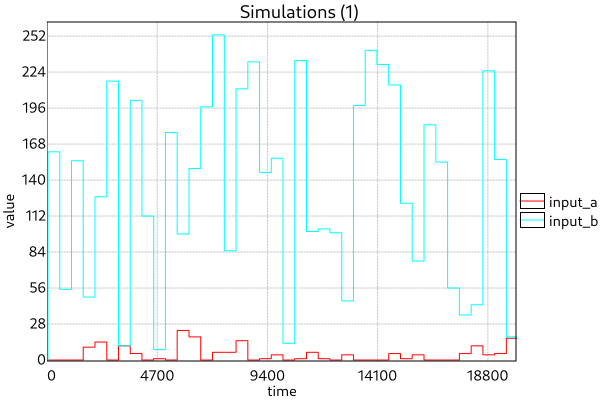
\includegraphics[width=0.95\linewidth]{obrazky-figures/inputs_beta_uni.png}
  \caption{Rozdělení \textbf{beta\_uni}}
  \label{fig:inputs_beta_uni}
\end{minipage}
\end{figure}

\begin{figure}[H]
\centering
\begin{minipage}{.5\textwidth}
  \centering
  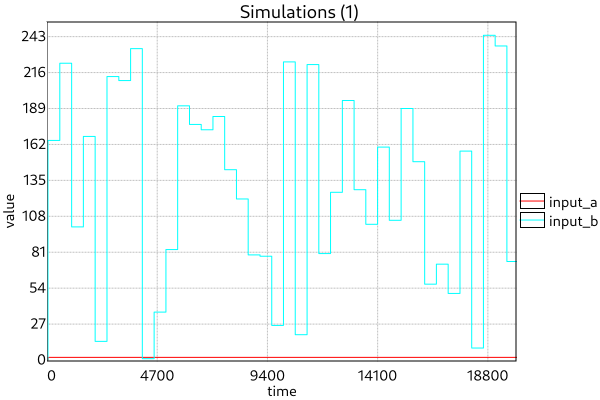
\includegraphics[width=0.95\linewidth]{obrazky-figures/inputs_const_norm.png}
  \caption{Rozdělení \textbf{const\_norm}}
  \label{fig:inputs_const_norm}
\end{minipage}%
\begin{minipage}{.5\textwidth}
  \centering
  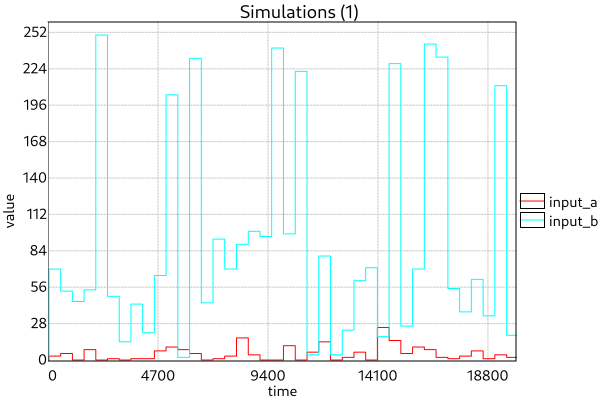
\includegraphics[width=0.95\linewidth]{obrazky-figures/inputs_gamma_2norm.png}
  \caption{Rozdělení \textbf{gamma\_2norm}}
  \label{fig:inputs_gamma_2norm}
\end{minipage}
\end{figure}

\begin{figure}[H]
\centering
\begin{minipage}{.5\textwidth}
  \centering
  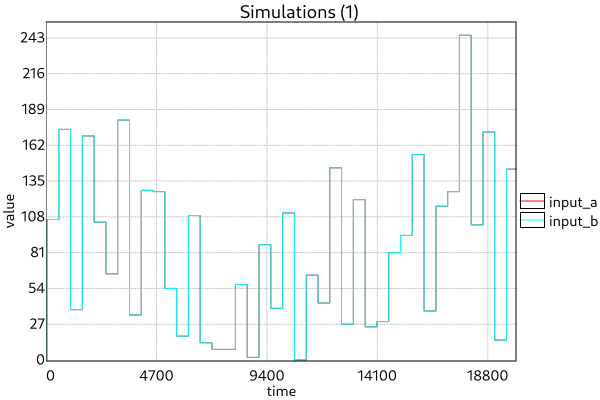
\includegraphics[width=0.95\linewidth]{obrazky-figures/inputs_same_triang.png}
  \caption{Rozdělení \textbf{same\_triang}}
  \label{fig:inputs_same_triang}
\end{minipage}%
\begin{minipage}{.5\textwidth}
  \centering
  \includegraphics[width=0.95\linewidth]{obrazky-figures/inputs_same_uni.png}
  \caption{Rozdělení \textbf{same\_uni}}
  \label{fig:inputs_same_uni}
\end{minipage}
\end{figure}

\begin{figure}[H]
\centering
\begin{minipage}{.5\textwidth}
  \centering
  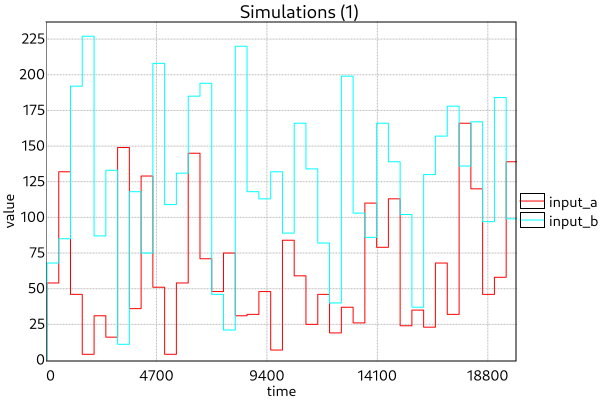
\includegraphics[width=0.95\linewidth]{obrazky-figures/inputs_triang_beta.png}
  \caption{Rozdělení \textbf{triang\_beta}}
  \label{fig:inputs_triang_beta}
\end{minipage}%
\begin{minipage}{.5\textwidth}
  \centering
  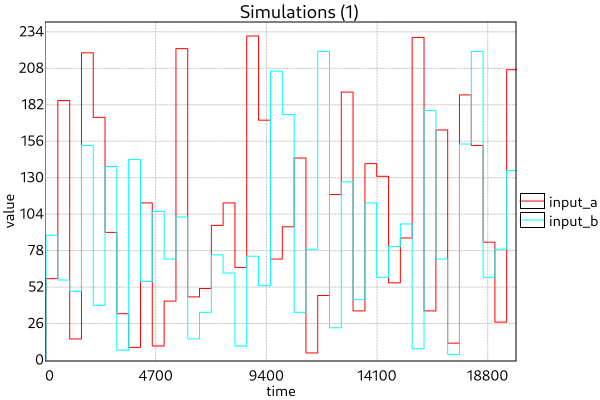
\includegraphics[width=0.95\linewidth]{obrazky-figures/inputs_triang_weibull.png}
  \caption{Rozdělení \textbf{triang\_weibull}}
  \label{fig:inputs_triang_weibull}
\end{minipage}
\end{figure}

\bigskip
\bigskip
\bigskip

\subsubsection{Porovnání přesných a přibližných výstupů}

\begin{figure}[H]
\centering
\begin{minipage}{.5\textwidth}
  \centering
  \includegraphics[width=0.95\linewidth]{obrazky-figures/results_R36.png}
  \caption{Násobička \textbf{mul8u\_R36}}
  \label{fig:results_R36}
\end{minipage}%
\begin{minipage}{.5\textwidth}
  \centering
  \includegraphics[width=0.95\linewidth]{obrazky-figures/results_17MN.png}
  \caption{Násobička \textbf{mul8u\_17MN}}
  \label{fig:results_17MN}
\end{minipage}
\end{figure}

\begin{figure}[H]
\centering
\begin{minipage}{.5\textwidth}
  \centering
  \includegraphics[width=0.95\linewidth]{obrazky-figures/results_1A0M.png}
  \caption{Násobička \textbf{mul8u\_1A0M}}
  \label{fig:results_1A0M}
\end{minipage}%
\begin{minipage}{.5\textwidth}
  \centering
  \includegraphics[width=0.95\linewidth]{obrazky-figures/results_12KA.png}
  \caption{Násobička \textbf{mul8u\_12KA}}
  \label{fig:results_12KA}
\end{minipage}
\end{figure}

\bigskip
\bigskip
\bigskip

\subsubsection{Sledování zpoždění}

\begin{figure}[H]
    \centering
    \includegraphics[width=0.6\textwidth]{obrazky-figures/delay_R36.png}
    \caption{Zpoždění násobičky \textbf{mul8u\_R36}}
    \label{fig:delay_R36}
\end{figure}

\begin{figure}[H]
    \centering
    \includegraphics[width=0.6\textwidth]{obrazky-figures/delay_12KA.png}
    \caption{Zpoždění násobičky \textbf{mul8u\_12KA}}
    \label{fig:delay_12KA}
\end{figure}

\begin{landscape}
\chapter{Podrobné výsledky experimentů} \label{append:exp_results}
\begin{table}[!ht]
    \centering
    \resizebox{1.5\textwidth}{!}{\begin{tabular}{|l|l|l|l|l|l|l|l|l|l|l|l|l|l|}
        \textbf{Násobička} & \textbf{Plocha} & \textbf{\% pokrytí} & \Centerstack{\textbf{Pravděpodobnost} \\ \textbf{chyby}} & \Centerstack{\textbf{Průměrná} \\ \textbf{absolutní} \\ \textbf{chyba}} & \Centerstack{\textbf{Průměrná} \\ \textbf{relativní} \\ \textbf{chyba}} & \Centerstack{\textbf{Průměrná} \\ \textbf{kvadratická} \\ \textbf{chyba}} & \Centerstack{\textbf{Nejhorší} \\ \textbf{absolutní} \\ \textbf{chyba}} & \Centerstack{\textbf{Nejhorší} \\ \textbf{relativní} \\ \textbf{chyba}} & \Centerstack{\textbf{Max.} \\ \textbf{Hammingova} \\ \textbf{vzdálenost}} & \Centerstack{\textbf{Průměrné} \\ \textbf{zpoždění}} & \Centerstack{\textbf{Nejhorší} \\ \textbf{zpoždění}} & \Centerstack{\textbf{Průměr} \\ \textbf{překl.} \\ \textbf{bitů}} & \Centerstack{\textbf{Max.} \\ \textbf{překl.} \\ \textbf{bitů}} \\ \hline
        mul8u\_17MN & 13.1 & 14.12 & 0.97 & 2342.61 & 0.59 & 42880774.66 & 17726.0 & 2.94 & 8.0 & 115.0 & 120.0 & 3.74 & 9.0 \\ 
        mul8u\_17MJ & 18.8 & 14.14 & 0.89 & 1406.84 & 0.53 & 28646249.92 & 17030.0 & 4.76 & 6.0 & 105.04 & 110.0 & 3.44 & 8.0 \\ 
        mul8u\_R36 & 60.5 & 14.13 & 0.98 & 3764.64 & 0.31 & 36718512.06 & 32289.0 & 1.0 & 10.0 & 338.56 & 380.0 & 12.76 & 30.0 \\  
        mul8u\_Z9D & 220.6 & 14.09 & 0.89 & 3141.56 & 0.16 & 32475721.88 & 31752.0 & 0.66 & 13.0 & 1290.61 & 1410.0 & 48.12 & 91.0 \\ 
        mul8u\_17R6 & 228.5 & 14.1 & 0.98 & 185.57 & 0.12 & 306809.19 & 1905.0 & 2.56 & 11.0 & 5162.93 & 6320.0 & 56.0 & 189.0 \\ 
        mul8u\_2NDH & 347.8 & 14.15 & 0.99 & 93.52 & 0.14 & 169105.55 & 2709.0 & 208.0 & 14.0 & 4263.88 & 4890.0 & 68.36 & 179.0 \\ 
        mul8u\_197B & 395.6 & 14.09 & 0.98 & 69.92 & 0.04 & 20974.73 & 424.0 & 1.0 & 14.0 & 9954.0 & 10650.0 & 124.19 & 312.0 \\ 
        mul8u\_NLX & 511.5 & 14.08 & 0.95 & 6.06 & 0.02 & 2751.55 & 161.0 & 1.29 & 14.0 & 12874.74 & 14430.0 & 163.53 & 421.0 \\ 
        mul8u\_GTR & 550.5 & 14.09 & 0.84 & 20.1 & 0.01 & 1528.88 & 125.0 & 1.0 & 13.0 & 13978.72 & 15470.0 & 176.54 & 459.0 \\ 
        mul8u\_BG1 & 561.8 & 14.13 & 0.49 & 289.01 & 0.03 & 393955.35 & 2932.0 & 0.53 & 13.0 & 19263.54 & 21750.0 & 184.4 & 555.0 \\ 
        mul8u\_R92 & 604.5 & 14.1 & 0.83 & 2.84 & 0.01 & 212.73 & 39.0 & 2.56 & 13.0 & 15563.89 & 17350.0 & 204.95 & 498.0 \\ 
        mul8u\_ZB3 & 682.8 & 14.15 & 0.07 & 0.14 & 0.0 & 0.27 & 2.0 & 0.22 & 10.0 & 17238.84 & 19040.0 & 230.85 & 538.0 \\ 
        mul8u\_12KA & 683.3 & 14.13 & 0.09 & 11.91 & 0.0 & 1761.59 & 192.0 & 0.28 & 9.0 & 16654.07 & 18160.0 & 223.03 & 511.0 \\ 
    \end{tabular}}
    \caption{Výsledky při generování vstupů s rozdělením uni\_uni}
    \label{uni_uni}
\end{table}

\begin{table}[!ht]
    \centering
    \resizebox{1.5\textwidth}{!}{\begin{tabular}{|l|l|l|l|l|l|l|l|l|l|l|l|l|l|}
        \textbf{Násobička} & \textbf{Plocha} & \textbf{\% pokrytí} & \Centerstack{\textbf{Pravděpodobnost} \\ \textbf{chyby}} & \Centerstack{\textbf{Průměrná} \\ \textbf{absolutní} \\ \textbf{chyba}} & \Centerstack{\textbf{Průměrná} \\ \textbf{relativní} \\ \textbf{chyba}} & \Centerstack{\textbf{Průměrná} \\ \textbf{kvadratická} \\ \textbf{chyba}} & \Centerstack{\textbf{Nejhorší} \\ \textbf{absolutní} \\ \textbf{chyba}} & \Centerstack{\textbf{Nejhorší} \\ \textbf{relativní} \\ \textbf{chyba}} & \Centerstack{\textbf{Max.} \\ \textbf{Hammingova} \\ \textbf{vzdálenost}} & \Centerstack{\textbf{Průměrné} \\ \textbf{zpoždění}} & \Centerstack{\textbf{Nejhorší} \\ \textbf{zpoždění}} & \Centerstack{\textbf{Průměr} \\ \textbf{překl.} \\ \textbf{bitů}} & \Centerstack{\textbf{Max.} \\ \textbf{překl.} \\ \textbf{bitů}} \\ \hline
        mul8u\_17MN & 13.1 & 5.74 & 0.53 & 403.82 & 0.63 & 642255.99 & 7719.0 & 1.0 & 4.0 & 114.97 & 120.0 & 0.0 & 0.0 \\ 
        mul8u\_17MJ & 18.8 & 5.7 & 0.32 & 386.49 & 0.62 & 597195.3 & 7470.0 & 2.02 & 2.0 & 104.94 & 110.0 & 0.0 & 3.0 \\ 
        mul8u\_R36 & 60.5 & 4.42 & 0.43 & 177.72 & 0.34 & 138906.19 & 3587.0 & 1.0 & 7.0 & 338.52 & 380.0 & 2.88 & 15.0 \\  
        mul8u\_Z9D & 220.6 & 5.84 & 0.24 & 46.86 & 0.04 & 25044.73 & 2544.0 & 0.46 & 11.0 & 1290.63 & 1440.0 & 20.32 & 73.0 \\ 
        mul8u\_17R6 & 228.5 & 5.69 & 0.6 & 112.54 & 0.47 & 63296.39 & 1058.0 & 1.02 & 8.0 & 5163.77 & 6350.0 & 3.72 & 58.0 \\ 
        mul8u\_2NDH & 347.8 & 5.74 & 0.63 & 42.81 & 2.33 & 17614.22 & 1286.0 & 208.0 & 12.0 & 4264.76 & 4940.0 & 8.54 & 60.0 \\ 
        mul8u\_197B & 395.6 & 5.75 & 0.62 & 55.24 & 0.28 & 9216.48 & 393.0 & 1.02 & 11.0 & 9952.51 & 10660.0 & 18.82 & 144.0 \\ 
        mul8u\_NLX & 511.5 & 5.79 & 0.59 & 19.07 & 0.14 & 1208.7 & 155.0 & 1.0 & 10.0 & 12872.55 & 14360.0 & 28.13 & 185.0 \\ 
        mul8u\_GTR & 550.5 & 5.77 & 0.57 & 16.57 & 0.14 & 951.67 & 125.0 & 1.0 & 10.0 & 13980.68 & 15520.0 & 32.09 & 224.0 \\ 
        mul8u\_BG1 & 561.8 & 5.8 & 0.2 & 46.56 & 0.04 & 27770.72 & 1780.0 & 0.53 & 10.0 & 19247.5 & 21830.0 & 36.47 & 186.0 \\ 
        mul8u\_R92 & 604.5 & 5.75 & 0.54 & 2.71 & 0.07 & 139.37 & 39.0 & 3.0 & 10.0 & 15571.76 & 17230.0 & 45.5 & 269.0 \\ 
        mul8u\_ZDF & 651.9 & 5.7 & 0.15 & 0.55 & 0.0 & 16.31 & 34.0 & 0.37 & 10.0 & 16358.54 & 18150.0 & 50.62 & 272.0 \\ 
        mul8u\_ZB3 & 682.8 & 5.77 & 0.03 & 0.07 & 0.0 & 0.13 & 2.0 & 0.22 & 9.0 & 17241.52 & 19190.0 & 55.97 & 294.0 \\ 
        mul8u\_12KA & 683.3 & 5.8 & 0.05 & 6.08 & 0.01 & 902.97 & 192.0 & 0.29 & 4.0 & 16663.53 & 18130.0 & 56.81 & 283.0 \\ 
    \end{tabular}}
    \caption{Výsledky při generování vstupů s rozdělením beta\_uni}
    \label{beta_uni}
\end{table}

\begin{table}[!ht]
    \centering
    \resizebox{1.5\textwidth}{!}{\begin{tabular}{|l|l|l|l|l|l|l|l|l|l|l|l|l|l|}
        \textbf{Násobička} & \textbf{Plocha} & \textbf{\% pokrytí} & \Centerstack{\textbf{Pravděpodobnost} \\ \textbf{chyby}} & \Centerstack{\textbf{Průměrná} \\ \textbf{absolutní} \\ \textbf{chyba}} & \Centerstack{\textbf{Průměrná} \\ \textbf{relativní} \\ \textbf{chyba}} & \Centerstack{\textbf{Průměrná} \\ \textbf{kvadratická} \\ \textbf{chyba}} & \Centerstack{\textbf{Nejhorší} \\ \textbf{absolutní} \\ \textbf{chyba}} & \Centerstack{\textbf{Nejhorší} \\ \textbf{relativní} \\ \textbf{chyba}} & \Centerstack{\textbf{Max.} \\ \textbf{Hammingova} \\ \textbf{vzdálenost}} & \Centerstack{\textbf{Průměrné} \\ \textbf{zpoždění}} & \Centerstack{\textbf{Nejhorší} \\ \textbf{zpoždění}} & \Centerstack{\textbf{Průměr} \\ \textbf{překl.} \\ \textbf{bitů}} & \Centerstack{\textbf{Max.} \\ \textbf{překl.} \\ \textbf{bitů}} \\ \hline
        mul8u\_17MN & 13.1 & 0.39 & 0.69 & 117.34 & 0.99 & 19667.2 & 508.0 & 1.0 & 3.0 & 114.99 & 120.0 & 0.0 & 0.0 \\ 
        mul8u\_17MJ & 18.8 & 0.39 & 0.34 & 115.63 & 0.99 & 19121.98 & 508.0 & 1.0 & 1.0 & 104.95 & 110.0 & 0.0 & 0.0 \\ 
        mul8u\_R36 & 60.5 & 0.38 & 0.75 & 62.46 & 0.71 & 5239.86 & 126.0 & 1.0 & 2.0 & 338.21 & 380.0 & 1.43 & 4.0 \\  
        mul8u\_Z9D & 220.6 & 0.39 & 0.0 & 0.0 & 0.0 & 0.0 & 0.0 & 0.0 & 0.0 & 1290.57 & 1410.0 & 13.65 & 32.0 \\ 
        mul8u\_17R6 & 228.5 & 0.39 & 0.94 & 116.76 & 0.99 & 19667.46 & 508.0 & 1.0 & 5.0 & 5168.19 & 6390.0 & 0.0 & 0.0 \\ 
        mul8u\_2NDH & 347.8 & 0.39 & 0.99 & 33.17 & 0.73 & 5188.43 & 126.0 & 1.0 & 6.0 & 4264.8 & 4940.0 & 2.97 & 10.0 \\ 
        mul8u\_197B & 395.6 & 0.39 & 0.99 & 80.78 & 0.82 & 7715.55 & 182.0 & 1.0 & 7.0 & 9952.15 & 10650.0 & 4.05 & 20.0 \\ 
        mul8u\_NLX & 511.5 & 0.39 & 0.93 & 24.41 & 0.36 & 975.7 & 62.0 & 1.0 & 4.0 & 12871.78 & 14340.0 & 9.97 & 33.0 \\ 
        mul8u\_GTR & 550.5 & 0.39 & 0.93 & 30.25 & 0.39 & 1254.22 & 62.0 & 1.0 & 4.0 & 13983.24 & 15550.0 & 11.81 & 37.0 \\ 
        mul8u\_BG1 & 561.8 & 0.39 & 0.0 & 0.0 & 0.0 & 0.0 & 0.0 & 0.0 & 0.0 & 19247.02 & 21780.0 & 23.51 & 58.0 \\ 
        mul8u\_R92 & 604.5 & 0.39 & 0.87 & 14.77 & 0.21 & 302.78 & 30.0 & 1.0 & 3.0 & 15564.57 & 17340.0 & 17.85 & 49.0 \\ 
        mul8u\_ZDF & 651.9 & 0.39 & 0.0 & 0.0 & 0.0 & 0.0 & 0.0 & 0.0 & 0.0 & 16359.14 & 18420.0 & 26.08 & 65.0 \\ 
        mul8u\_ZB3 & 682.8 & 0.39 & 0.0 & 0.0 & 0.0 & 0.0 & 0.0 & 0.0 & 0.0 & 17234.96 & 19160.0 & 27.95 & 69.0 \\ 
        mul8u\_12KA & 683.3 & 0.39 & 0.0 & 0.0 & 0.0 & 0.0 & 0.0 & 0.0 & 0.0 & 16672.32 & 18400.0 & 28.33 & 70.0 \\ 
    \end{tabular}}
    \caption{Výsledky při generování vstupů s rozdělením const\_norm}
    \label{const_norm}
\end{table}

\begin{table}[!ht]
    \centering
    \resizebox{1.5\textwidth}{!}{\begin{tabular}{|l|l|l|l|l|l|l|l|l|l|l|l|l|l|}
        \textbf{Násobička} & \textbf{Plocha} & \textbf{\% pokrytí} & \Centerstack{\textbf{Pravděpodobnost} \\ \textbf{chyby}} & \Centerstack{\textbf{Průměrná} \\ \textbf{absolutní} \\ \textbf{chyba}} & \Centerstack{\textbf{Průměrná} \\ \textbf{relativní} \\ \textbf{chyba}} & \Centerstack{\textbf{Průměrná} \\ \textbf{kvadratická} \\ \textbf{chyba}} & \Centerstack{\textbf{Nejhorší} \\ \textbf{absolutní} \\ \textbf{chyba}} & \Centerstack{\textbf{Nejhorší} \\ \textbf{relativní} \\ \textbf{chyba}} & \Centerstack{\textbf{Max.} \\ \textbf{Hammingova} \\ \textbf{vzdálenost}} & \Centerstack{\textbf{Průměrné} \\ \textbf{zpoždění}} & \Centerstack{\textbf{Nejhorší} \\ \textbf{zpoždění}} & \Centerstack{\textbf{Průměr} \\ \textbf{překl.} \\ \textbf{bitů}} & \Centerstack{\textbf{Max.} \\ \textbf{překl.} \\ \textbf{bitů}} \\ \hline
        mul8u\_17MN & 13.1 & 4.9 & 0.67 & 510.49 & 0.83 & 1022758.54 & 10665.0 & 1.0 & 5.0 & 115.02 & 120.0 & 0.0 & 0.0 \\ 
        mul8u\_17MJ & 18.8 & 4.93 & 0.41 & 521.55 & 0.83 & 1033542.01 & 8280.0 & 5.12 & 4.0 & 105.01 & 110.0 & 0.01 & 3.0 \\ 
        mul8u\_R36 & 60.5 & 4.01 & 0.63 & 249.63 & 0.55 & 196629.08 & 3888.0 & 1.0 & 8.0 & 338.09 & 380.0 & 3.21 & 16.0 \\  
        mul8u\_Z9D & 220.6 & 4.91 & 0.35 & 74.28 & 0.06 & 55009.73 & 4864.0 & 0.48 & 9.0 & 1290.75 & 1420.0 & 24.22 & 78.0 \\ 
        mul8u\_17R6 & 228.5 & 4.9 & 0.8 & 154.84 & 0.65 & 79586.26 & 1185.0 & 1.02 & 8.0 & 5165.0 & 6350.0 & 4.63 & 74.0 \\ 
        mul8u\_2NDH & 347.8 & 4.91 & 0.83 & 71.8 & 1.77 & 32365.21 & 1301.0 & 208.0 & 12.0 & 4264.34 & 4950.0 & 11.01 & 70.0 \\ 
        mul8u\_197B & 395.6 & 4.94 & 0.83 & 70.8 & 0.42 & 11724.64 & 403.0 & 1.02 & 11.0 & 9951.55 & 10770.0 & 23.15 & 179.0 \\ 
        mul8u\_NLX & 511.5 & 4.97 & 0.79 & 25.49 & 0.24 & 1741.28 & 155.0 & 1.35 & 10.0 & 12872.99 & 14310.0 & 34.84 & 225.0 \\ 
        mul8u\_GTR & 550.5 & 4.97 & 0.75 & 21.21 & 0.21 & 1276.35 & 125.0 & 1.0 & 10.0 & 13978.34 & 15540.0 & 39.66 & 226.0 \\ 
        mul8u\_BG1 & 561.8 & 4.96 & 0.29 & 70.92 & 0.06 & 51509.66 & 1786.0 & 0.53 & 11.0 & 19254.78 & 21870.0 & 44.54 & 203.0 \\ 
        mul8u\_R92 & 604.5 & 4.95 & 0.72 & 3.77 & 0.11 & 187.57 & 39.0 & 3.0 & 9.0 & 15561.95 & 17390.0 & 57.73 & 362.0 \\ 
        mul8u\_ZDF & 651.9 & 4.92 & 0.22 & 0.67 & 0.01 & 25.3 & 34.0 & 0.37 & 9.0 & 16357.23 & 18200.0 & 65.03 & 263.0 \\ 
        mul8u\_ZB3 & 682.8 & 4.97 & 0.05 & 0.09 & 0.0 & 0.18 & 2.0 & 0.22 & 9.0 & 17234.22 & 19250.0 & 72.47 & 311.0 \\ 
        mul8u\_12KA & 683.3 & 5.01 & 0.06 & 10.21 & 0.01 & 1725.25 & 192.0 & 0.29 & 6.0 & 16663.23 & 18240.0 & 72.02 & 301.0 \\ 
    \end{tabular}}
    \caption{Výsledky při generování vstupů s rozdělením gamma\_2norm}
    \label{gamma_2norm}
\end{table}

\begin{table}[!ht]
    \centering
    \resizebox{1.5\textwidth}{!}{\begin{tabular}{|l|l|l|l|l|l|l|l|l|l|l|l|l|l|}
        \textbf{Násobička} & \textbf{Plocha} & \textbf{\% pokrytí} & \Centerstack{\textbf{Pravděpodobnost} \\ \textbf{chyby}} & \Centerstack{\textbf{Průměrná} \\ \textbf{absolutní} \\ \textbf{chyba}} & \Centerstack{\textbf{Průměrná} \\ \textbf{relativní} \\ \textbf{chyba}} & \Centerstack{\textbf{Průměrná} \\ \textbf{kvadratická} \\ \textbf{chyba}} & \Centerstack{\textbf{Nejhorší} \\ \textbf{absolutní} \\ \textbf{chyba}} & \Centerstack{\textbf{Nejhorší} \\ \textbf{relativní} \\ \textbf{chyba}} & \Centerstack{\textbf{Max.} \\ \textbf{Hammingova} \\ \textbf{vzdálenost}} & \Centerstack{\textbf{Průměrné} \\ \textbf{zpoždění}} & \Centerstack{\textbf{Nejhorší} \\ \textbf{zpoždění}} & \Centerstack{\textbf{Průměr} \\ \textbf{překl.} \\ \textbf{bitů}} & \Centerstack{\textbf{Max.} \\ \textbf{překl.} \\ \textbf{bitů}} \\ \hline
        mul8u\_17MN & 13.1 & 0.39 & 0.87 & 995.26 & 0.72 & 32130790.77 & 17533.0 & 1.01 & 7.0 & 114.93 & 120.0 & 2.33 & 9.0 \\ 
        mul8u\_17MJ & 18.8 & 0.39 & 0.83 & 910.72 & 0.93 & 21805715.51 & 17284.0 & 5.12 & 6.0 & 105.05 & 110.0 & 2.64 & 8.0 \\  
        mul8u\_Z9D & 220.6 & 0.39 & 0.93 & 2637.22 & 0.22 & 23174748.65 & 31752.0 & 0.49 & 11.0 & 1290.6 & 1420.0 & 43.41 & 99.0 \\ 
        mul8u\_17R6 & 228.5 & 0.39 & 0.89 & 298.75 & 0.28 & 295517.54 & 1469.0 & 1.0 & 9.0 & 5162.99 & 6390.0 & 37.58 & 196.0 \\ 
        mul8u\_2NDH & 347.8 & 0.38 & 0.96 & 131.36 & 0.64 & 150980.9 & 2056.0 & 208.0 & 12.0 & 4263.55 & 4880.0 & 51.69 & 183.0 \\ 
        mul8u\_197B & 395.6 & 0.39 & 0.95 & 80.62 & 0.14 & 25775.88 & 399.0 & 1.0 & 12.0 & 9955.21 & 10710.0 & 97.21 & 299.0 \\ 
        mul8u\_NLX & 511.5 & 0.39 & 0.9 & 5.89 & 0.08 & 4419.01 & 161.0 & 1.0 & 10.0 & 12862.65 & 14350.0 & 129.08 & 420.0 \\ 
        mul8u\_GTR & 550.5 & 0.39 & 0.84 & 25.34 & 0.07 & 1822.18 & 105.0 & 1.0 & 9.0 & 13975.3 & 15560.0 & 142.56 & 423.0 \\ 
        mul8u\_BG1 & 561.8 & 0.39 & 0.54 & 231.18 & 0.03 & 400613.36 & 2938.0 & 0.37 & 10.0 & 19263.65 & 21800.0 & 147.81 & 488.0 \\ 
        mul8u\_R92 & 604.5 & 0.39 & 0.75 & 0.63 & 0.03 & 153.83 & 34.0 & 1.0 & 9.0 & 15562.17 & 17250.0 & 172.48 & 500.0 \\ 
        mul8u\_ZDF & 651.9 & 0.39 & 0.58 & 0.32 & 0.01 & 105.93 & 28.0 & 0.37 & 13.0 & 16352.29 & 18230.0 & 184.83 & 503.0 \\ 
        mul8u\_ZB3 & 682.8 & 0.39 & 0.25 & 0.49 & 0.0 & 0.98 & 2.0 & 0.22 & 8.0 & 17236.71 & 19340.0 & 196.22 & 569.0 \\ 
        mul8u\_12KA & 683.3 & 0.39 & 0.05 & 4.48 & 0.0 & 463.0 & 192.0 & 0.01 & 6.0 & 16659.01 & 18230.0 & 196.87 & 512.0 \\ 
    \end{tabular}}
    \caption{Výsledky při generování vstupů s rozdělením same\_triang}
    \label{same_triang}
\end{table}

\begin{table}[!ht]
    \centering
    \resizebox{1.5\textwidth}{!}{\begin{tabular}{|l|l|l|l|l|l|l|l|l|l|l|l|l|l|}
        \textbf{Násobička} & \textbf{Plocha} & \textbf{\% pokrytí} & \Centerstack{\textbf{Pravděpodobnost} \\ \textbf{chyby}} & \Centerstack{\textbf{Průměrná} \\ \textbf{absolutní} \\ \textbf{chyba}} & \Centerstack{\textbf{Průměrná} \\ \textbf{relativní} \\ \textbf{chyba}} & \Centerstack{\textbf{Průměrná} \\ \textbf{kvadratická} \\ \textbf{chyba}} & \Centerstack{\textbf{Nejhorší} \\ \textbf{absolutní} \\ \textbf{chyba}} & \Centerstack{\textbf{Nejhorší} \\ \textbf{relativní} \\ \textbf{chyba}} & \Centerstack{\textbf{Max.} \\ \textbf{Hammingova} \\ \textbf{vzdálenost}} & \Centerstack{\textbf{Průměrné} \\ \textbf{zpoždění}} & \Centerstack{\textbf{Nejhorší} \\ \textbf{zpoždění}} & \Centerstack{\textbf{Průměr} \\ \textbf{překl.} \\ \textbf{bitů}} & \Centerstack{\textbf{Max.} \\ \textbf{překl.} \\ \textbf{bitů}} \\ \hline
        mul8u\_17MN & 13.1 & 0.39 & 0.93 & 1606.1 & 0.53 & 48959181.88 & 17533.0 & 1.01 & 7.0 & 114.98 & 120.0 & 3.77 & 9.0 \\ 
        mul8u\_17MJ & 18.8 & 0.39 & 0.89 & 2130.75 & 0.66 & 34300636.73 & 17793.0 & 5.12 & 6.0 & 105.06 & 110.0 & 3.86 & 8.0 \\ 
        mul8u\_R36 & 60.5 & 0.39 & 0.97 & 6731.84 & 0.36 & 111108008.89 & 32289.0 & 1.0 & 8.0 & 338.23 & 380.0 & 12.61 & 30.0 \\  
        mul8u\_Z9D & 220.6 & 0.39 & 0.97 & 6560.92 & 0.25 & 108295128.03 & 32258.0 & 0.5 & 11.0 & 1290.64 & 1410.0 & 48.32 & 113.0 \\ 
        mul8u\_17R6 & 228.5 & 0.39 & 0.93 & 265.58 & 0.17 & 334967.5 & 1469.0 & 1.0 & 9.0 & 5170.15 & 6310.0 & 61.07 & 217.0 \\ 
        mul8u\_2NDH & 347.8 & 0.39 & 0.98 & 190.35 & 0.22 & 304076.77 & 2565.0 & 208.0 & 12.0 & 4261.22 & 4940.0 & 69.75 & 186.0 \\ 
        mul8u\_197B & 395.6 & 0.39 & 0.97 & 68.63 & 0.09 & 26932.71 & 399.0 & 1.0 & 12.0 & 9952.21 & 10860.0 & 126.55 & 344.0 \\ 
        mul8u\_NLX & 511.5 & 0.39 & 0.93 & 1.75 & 0.05 & 4415.26 & 161.0 & 1.0 & 10.0 & 12861.77 & 14410.0 & 165.21 & 412.0 \\ 
        mul8u\_GTR & 550.5 & 0.39 & 0.85 & 22.04 & 0.04 & 1649.62 & 105.0 & 1.0 & 9.0 & 13975.75 & 15690.0 & 180.46 & 433.0 \\ 
        mul8u\_BG1 & 561.8 & 0.39 & 0.59 & 332.9 & 0.02 & 513636.13 & 2938.0 & 0.37 & 10.0 & 19266.83 & 21900.0 & 188.28 & 563.0 \\ 
        mul8u\_R92 & 604.5 & 0.39 & 0.77 & 0.09 & 0.02 & 158.92 & 34.0 & 1.0 & 9.0 & 15568.66 & 17320.0 & 211.04 & 509.0 \\ 
        mul8u\_ZDF & 651.9 & 0.39 & 0.6 & 0.62 & 0.01 & 108.98 & 28.0 & 0.37 & 13.0 & 16353.46 & 18250.0 & 225.07 & 517.0 \\ 
        mul8u\_ZB3 & 682.8 & 0.39 & 0.25 & 0.5 & 0.0 & 0.99 & 2.0 & 0.22 & 9.0 & 17234.77 & 19150.0 & 236.42 & 565.0 \\ 
        mul8u\_12KA & 683.3 & 0.39 & 0.1 & 12.64 & 0.0 & 1881.38 & 192.0 & 0.01 & 6.0 & 16660.82 & 18230.0 & 235.51 & 536.0 \\ 
    \end{tabular}}
    \caption{Výsledky při generování vstupů s rozdělením same\_uni}
    \label{same_uni}
\end{table}

\begin{table}[!ht]
    \centering
    \resizebox{1.5\textwidth}{!}{\begin{tabular}{|l|l|l|l|l|l|l|l|l|l|l|l|l|l|}
        \textbf{Násobička} & \textbf{Plocha} & \textbf{\% pokrytí} & \Centerstack{\textbf{Pravděpodobnost} \\ \textbf{chyby}} & \Centerstack{\textbf{Průměrná} \\ \textbf{absolutní} \\ \textbf{chyba}} & \Centerstack{\textbf{Průměrná} \\ \textbf{relativní} \\ \textbf{chyba}} & \Centerstack{\textbf{Průměrná} \\ \textbf{kvadratická} \\ \textbf{chyba}} & \Centerstack{\textbf{Nejhorší} \\ \textbf{absolutní} \\ \textbf{chyba}} & \Centerstack{\textbf{Nejhorší} \\ \textbf{relativní} \\ \textbf{chyba}} & \Centerstack{\textbf{Max.} \\ \textbf{Hammingova} \\ \textbf{vzdálenost}} & \Centerstack{\textbf{Průměrné} \\ \textbf{zpoždění}} & \Centerstack{\textbf{Nejhorší} \\ \textbf{zpoždění}} & \Centerstack{\textbf{Průměr} \\ \textbf{překl.} \\ \textbf{bitů}} & \Centerstack{\textbf{Max.} \\ \textbf{překl.} \\ \textbf{bitů}} \\ \hline
        mul8u\_17MN & 13.1 & 24.47 & 0.94 & 1908.7 & 0.58 & 44016175.32 & 17662.0 & 2.88 & 8.0 & 115.03 & 120.0 & 3.4 & 9.0 \\ 
        mul8u\_17MJ & 18.8 & 24.65 & 0.88 & 1130.23 & 0.5 & 27626212.71 & 16384.0 & 4.94 & 6.0 & 104.98 & 110.0 & 3.2 & 8.0 \\ 
        mul8u\_R36 & 60.5 & 24.56 & 0.94 & 2846.44 & 0.26 & 19135040.46 & 28280.0 & 1.0 & 10.0 & 338.5 & 380.0 & 12.2 & 30.0 \\  
        mul8u\_Z9D & 220.6 & 24.7 & 0.86 & 2193.26 & 0.13 & 15285448.93 & 29480.0 & 0.49 & 13.0 & 1290.58 & 1420.0 & 47.03 & 91.0 \\ 
        mul8u\_17R6 & 228.5 & 24.65 & 0.94 & 181.07 & 0.08 & 311500.42 & 1925.0 & 2.16 & 12.0 & 5171.66 & 6490.0 & 52.38 & 198.0 \\ 
        mul8u\_2NDH & 347.8 & 24.63 & 0.96 & 81.97 & 0.6 & 136136.6 & 2117.0 & 208.0 & 14.0 & 4263.25 & 4880.0 & 64.3 & 170.0 \\ 
        mul8u\_197B & 395.6 & 24.59 & 0.94 & 68.81 & 0.03 & 20687.88 & 431.0 & 1.02 & 15.0 & 9953.64 & 10700.0 & 117.1 & 298.0 \\ 
        mul8u\_NLX & 511.5 & 24.58 & 0.91 & 5.29 & 0.01 & 2629.8 & 161.0 & 1.0 & 15.0 & 12872.46 & 14500.0 & 153.74 & 393.0 \\ 
        mul8u\_GTR & 550.5 & 24.62 & 0.81 & 19.56 & 0.01 & 1490.17 & 125.0 & 1.0 & 12.0 & 13980.94 & 15520.0 & 167.76 & 429.0 \\ 
        mul8u\_BG1 & 561.8 & 24.71 & 0.48 & 272.05 & 0.03 & 390470.61 & 2938.0 & 0.52 & 13.0 & 19264.64 & 21830.0 & 172.46 & 547.0 \\ 
        mul8u\_R92 & 604.5 & 24.44 & 0.8 & 2.87 & 0.0 & 204.07 & 39.0 & 1.0 & 15.0 & 15565.35 & 17320.0 & 193.87 & 489.0 \\ 
        mul8u\_ZDF & 651.9 & 24.55 & 0.38 & 0.69 & 0.0 & 56.85 & 34.0 & 0.18 & 13.0 & 16359.27 & 18250.0 & 205.36 & 497.0 \\ 
        mul8u\_ZB3 & 682.8 & 24.5 & 0.06 & 0.12 & 0.0 & 0.23 & 2.0 & 0.04 & 10.0 & 17221.87 & 19090.0 & 216.34 & 569.0 \\ 
        mul8u\_12KA & 683.3 & 24.51 & 0.08 & 8.23 & 0.0 & 977.34 & 192.0 & 0.27 & 10.0 & 16667.06 & 18410.0 & 214.11 & 491.0 \\ 
    \end{tabular}}
    \caption{Výsledky při generování vstupů s rozdělením triang\_beta}
    \label{triang_beta}
\end{table}

\begin{table}[!ht]
    \centering
    \resizebox{1.5\textwidth}{!}{\begin{tabular}{|l|l|l|l|l|l|l|l|l|l|l|l|l|l|}
        \textbf{Násobička} & \textbf{Plocha} & \textbf{\% pokrytí} & \Centerstack{\textbf{Pravděpodobnost} \\ \textbf{chyby}} & \Centerstack{\textbf{Průměrná} \\ \textbf{absolutní} \\ \textbf{chyba}} & \Centerstack{\textbf{Průměrná} \\ \textbf{relativní} \\ \textbf{chyba}} & \Centerstack{\textbf{Průměrná} \\ \textbf{kvadratická} \\ \textbf{chyba}} & \Centerstack{\textbf{Nejhorší} \\ \textbf{absolutní} \\ \textbf{chyba}} & \Centerstack{\textbf{Nejhorší} \\ \textbf{relativní} \\ \textbf{chyba}} & \Centerstack{\textbf{Max.} \\ \textbf{Hammingova} \\ \textbf{vzdálenost}} & \Centerstack{\textbf{Průměrné} \\ \textbf{zpoždění}} & \Centerstack{\textbf{Nejhorší} \\ \textbf{zpoždění}} & \Centerstack{\textbf{Průměr} \\ \textbf{překl.} \\ \textbf{bitů}} & \Centerstack{\textbf{Max.} \\ \textbf{překl.} \\ \textbf{bitů}} \\ \hline
        mul8u\_17MN & 13.1 & 24.07 & 0.96 & 2714.61 & 0.78 & 32971527.69 & 17789.0 & 2.94 & 8.0 & 114.97 & 120.0 & 2.45 & 9.0 \\ 
        mul8u\_17MJ & 18.8 & 24.01 & 0.85 & 1594.32 & 0.74 & 21622768.14 & 16384.0 & 5.12 & 6.0 & 105.03 & 110.0 & 2.39 & 8.0 \\ 
        mul8u\_R36 & 60.5 & 1.81 & 0.65 & 2121.24 & 0.33 & 11793979.69 & 27360.0 & 1.0 & 9.0 & 338.35 & 380.0 & 6.96 & 26.0 \\  
        mul8u\_Z9D & 220.6 & 24.04 & 0.84 & 1276.01 & 0.13 & 6554886.95 & 27996.0 & 0.51 & 12.0 & 1290.19 & 1420.0 & 44.77 & 91.0 \\ 
        mul8u\_17R6 & 228.5 & 24.01 & 0.97 & 208.34 & 0.19 & 293170.32 & 1867.0 & 2.56 & 11.0 & 5160.37 & 6390.0 & 37.88 & 184.0 \\ 
        mul8u\_2NDH & 347.8 & 24.09 & 0.99 & 69.75 & 0.22 & 90747.81 & 2709.0 & 208.0 & 15.0 & 4263.95 & 4940.0 & 54.05 & 169.0 \\ 
        mul8u\_197B & 395.6 & 24.08 & 0.98 & 82.02 & 0.07 & 21982.34 & 431.0 & 1.02 & 15.0 & 9952.92 & 10670.0 & 101.53 & 303.0 \\ 
        mul8u\_NLX & 511.5 & 24.08 & 0.95 & 9.55 & 0.03 & 2815.48 & 161.0 & 1.0 & 12.0 & 12871.16 & 14370.0 & 137.21 & 428.0 \\ 
        mul8u\_GTR & 550.5 & 24.11 & 0.84 & 21.49 & 0.02 & 1548.65 & 125.0 & 1.0 & 12.0 & 13982.51 & 15600.0 & 148.85 & 409.0 \\ 
        mul8u\_BG1 & 561.8 & 23.95 & 0.44 & 192.93 & 0.03 & 286195.05 & 2932.0 & 0.53 & 13.0 & 19251.81 & 21730.0 & 153.4 & 502.0 \\ 
        mul8u\_R92 & 604.5 & 24.05 & 0.83 & 3.39 & 0.01 & 210.75 & 39.0 & 2.56 & 14.0 & 15559.05 & 17250.0 & 177.41 & 448.0 \\ 
        mul8u\_ZDF & 651.9 & 23.96 & 0.4 & 0.6 & 0.0 & 60.71 & 34.0 & 0.29 & 14.0 & 16355.83 & 18180.0 & 189.4 & 542.0 \\ 
        mul8u\_ZB3 & 682.8 & 24.03 & 0.06 & 0.12 & 0.0 & 0.24 & 2.0 & 0.04 & 11.0 & 17219.58 & 19110.0 & 201.25 & 523.0 \\ 
        mul8u\_12KA & 683.3 & 24.12 & 0.05 & 4.42 & 0.0 & 426.44 & 192.0 & 0.22 & 9.0 & 16665.62 & 18200.0 & 197.97 & 491.0 \\ 
    \end{tabular}}
    \caption{Výsledky při generování vstupů s rozdělením triang\_weibull}
    \label{triang_weibull}
\end{table}

\end{landscape}